\chapter{Kwantumgetallen en elektronenconfiguraties}\label{ch:b1:quantum-numbers}

Vul een glazen buis met waterstof onder lage druk, stuur er een
elektrische ontlading door en bekijk de roze gloed door een prisma. Het
licht wordt niet uitgespreid tot een regenboog. Het valt uiteen in vier
scherpe lijnen --- één rode, één blauwgroene, twee violette --- en
daartussen niets. Een hete vaste stof straalt bij alle golflengten; een
waterstofatoom zendt er maar een handvol uit. De verklaring, gevonden
tussen 1913 en 1926, is dat de energie van een elektron in een atoom niet
elke waarde kan aannemen: ze is \emph{gekwantiseerd}. Dit hoofdstuk geeft
de regels van die kwantisering zoals een chemicus ze gebruikt --- vier
kwantumgetallen, drie opvulregels --- en leidt daaruit de
\omterm{def:b1:quantum-numbers:configuration}{elektronenconfiguratie} van elk atoom en elk ion af, de sleutel tot het
periodiek systeem van het volgende hoofdstuk.

\begin{recall}
Boek 1 (jaar 10) verdeelde de elektronen van de eerste twintig elementen
over schillen en \omterm{def:b1:quantum-numbers:orbital}{subschillen}, 1s, 2s, 2p, 3s, 3p, en noemde de elektronen
van de buitenste schil de \omterm{def:b1:quantum-numbers:configuration}{valentie-elektronen}. Uit de natuurkunde
gebruiken we als bekend dat licht met golflengte $\lambda$ bestaat uit
fotonen met energie $E = h\nu = hc/\lambda$, waarin $h$ de constante van
Planck is en $c$ de lichtsnelheid.
\end{recall}

\begin{omfigure}
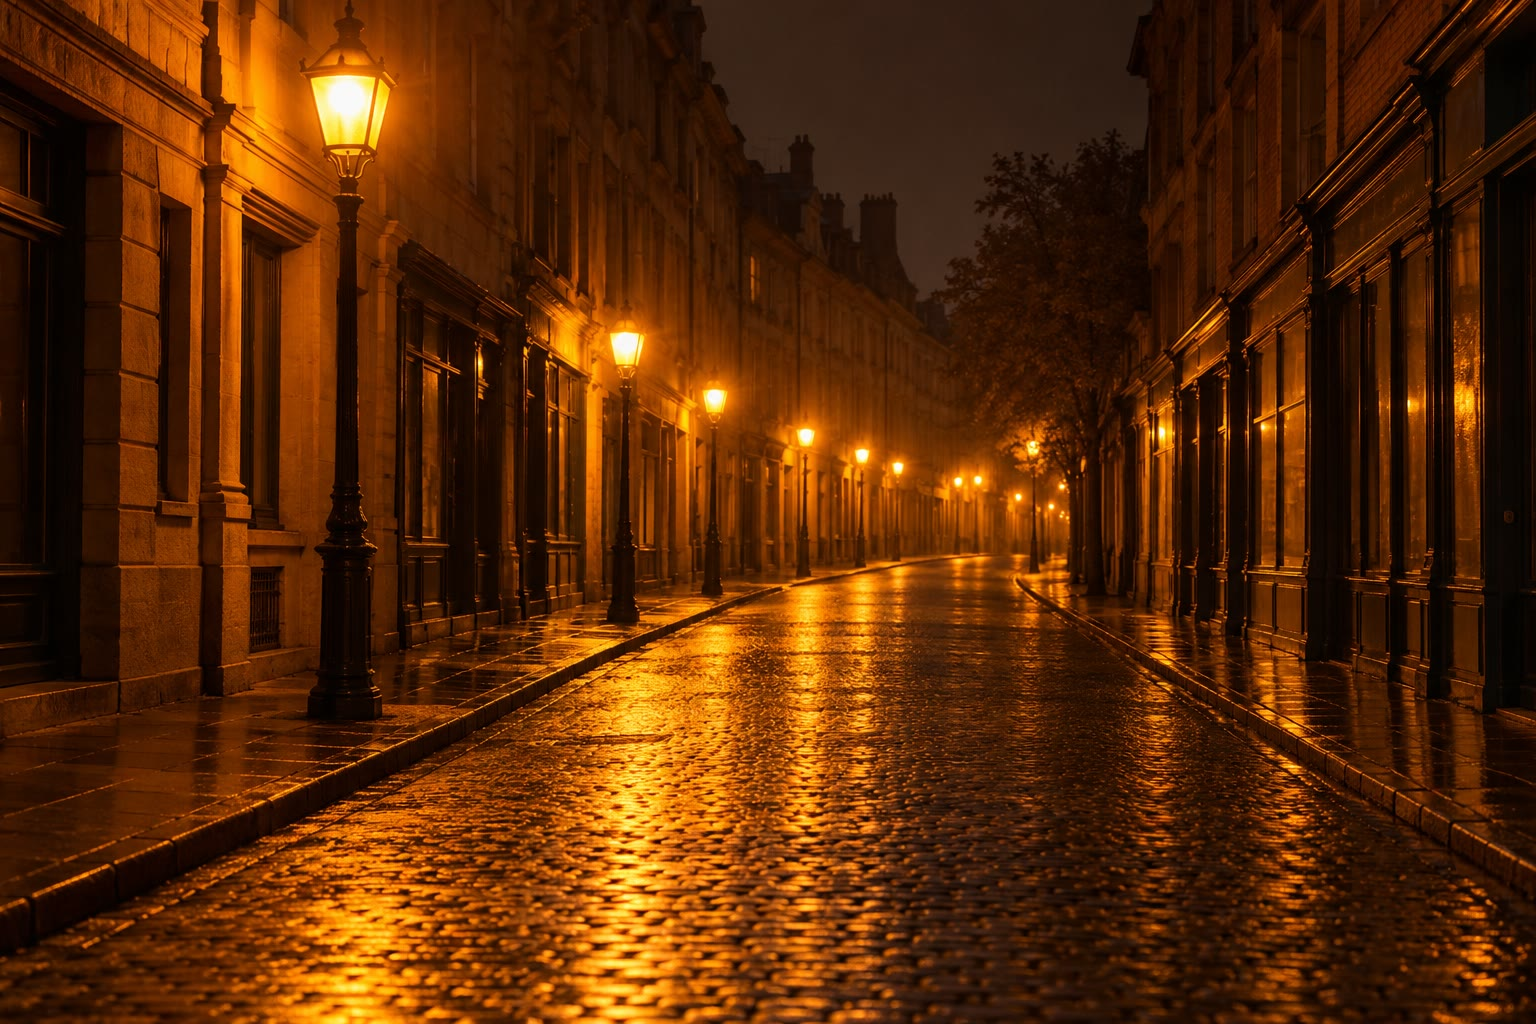
\includegraphics[width=0.62\linewidth]{images/book2/ai/b1-01-street-lamps.jpg}

{\small Lagedruknatriumlampen langs een straat. Hun licht is bijna één
enkele oranjegele lijn: net als waterstof zendt een aangeslagen
natriumatoom alleen fotonen met een paar welbepaalde energieën uit.}
\end{omfigure}

\section{Gekwantiseerde energieën: het spectrum van waterstof}

\begin{definition}[Energieniveau, grondtoestand, aangeslagen toestand]\label{def:b1:quantum-numbers:energy-level}
De energie van een elektron dat in een atoom gebonden is, kan alleen
bepaalde waarden aannemen: de \emph{energieniveaus}\index{energieniveau}
van het atoom. Het nulpunt van de energie ligt bij een elektron dat in
rust is, oneindig ver van de kern (het atoom is geïoniseerd), zodat elk
niveau van een gebonden elektron negatief is. Het laagste niveau is de
\emph{grondtoestand}\index{grondtoestand}; elk ander niveau is een
\emph{aangeslagen toestand}\index{aangeslagen toestand}.
\end{definition}

Een atoom gaat van een niveau met energie $E_{\text{hoog}}$ naar een lager
niveau $E_{\text{laag}}$ door één foton uit te zenden, en van het lagere
naar het hogere niveau door er één te absorberen, met energie
\[
  h\nu = \frac{hc}{\lambda} = E_{\text{hoog}} - E_{\text{laag}} .
\]
Een lijnenspectrum is dus een afbeelding van de verschillen tussen de
niveaus.

\begin{theorem}[Energieniveaus van het waterstofatoom]\label{thm:b1:quantum-numbers:levels}
De \omterm{def:b1:quantum-numbers:energy-level}{energieniveaus} van het waterstofatoom zijn
\[
  E_n = -\frac{E_R}{n^2}, \qquad n = 1, 2, 3, \dots,
  \qquad E_R = \qty{13.6}{eV},
\]
waarin $E_R$ de rydbergenergie is (gecorrigeerd voor de beweging van de
kern). De \omterm{def:b1:quantum-numbers:energy-level}{grondtoestand} is $E_1 = \qty{-13.6}{eV}$ en de
ionisatie-energie van het atoom is $E_R$.
% ledger: const:RyhcEV, ie:H (13.598 eV; levels computed in
% figdata/bachelor-1/hydrogen-levels.py)
\end{theorem}
\admitted

\begin{remark}[Waar de formule vandaan komt]\label{rem:b1:quantum-numbers:schrodinger}
De formule volgt uit het oplossen van de schrödingervergelijking van het
elektron in het veld van het proton; die oplossing, en de vormen van de
golffuncties die ze oplevert, worden afgeleid in het deel van jaar 2.
Niels Bohr had in 1913 dezelfde niveaus gevonden met een eenvoudiger
model van cirkelbanen, dat inmiddels verlaten is.
\end{remark}

\begin{proposition}[De formule van Rydberg]\label{prop:b1:quantum-numbers:rydberg}
De lijnen die waterstof uitzendt, hebben golflengten gegeven door
\[
  \frac{1}{\lambda} = R_H\left(\frac{1}{n_1^2} - \frac{1}{n_2^2}\right),
  \qquad n_2 > n_1 \ge 1, \qquad R_H = \frac{E_R}{hc},
\]
voor de overgang van niveau $n_2$ naar niveau $n_1$. De lijnen die op
hetzelfde niveau $n_1$ eindigen, vormen een \emph{reeks}: Lyman voor
$n_1 = 1$ (ultraviolet), Balmer voor $n_1 = 2$ (zichtbaar), Paschen voor
$n_1 = 3$ (infrarood).
\end{proposition}

\begin{proof}
Het foton draagt de energie weg die het atoom verliest:
$hc/\lambda = E_{n_2} - E_{n_1} = -E_R/n_2^2 + E_R/n_1^2
= E_R\,(1/n_1^2 - 1/n_2^2)$. Delen door $hc$ geeft de formule.
\end{proof}

\begin{example}[De rode lijn van waterstof]\label{ex:b1:quantum-numbers:halpha}
Voor de overgang $3 \to 2$: $\Delta E = 13.6\,(1/4 - 1/9) =
\qty{1.89}{eV}$. Met $hc = \qty{1240}{eV.nm}$ (uit de waarden van $h$,
$c$ en $e$) is $\lambda = 1240/1.89 = \qty{656}{nm}$: de rode lijn.
De andere balmerlijnen, $4 \to 2$, $5 \to 2$, $6 \to 2$, liggen bij 486,
434 en \qty{410}{nm}; de volgende, $7 \to 2$ bij \qty{397}{nm}, ligt al
in het ultraviolet. De gemeten golflengten, 656.3, 486.1, 434.0 en
\qty{410.2}{nm}, stemmen hiermee overeen tot op minder dan één op
tweeduizend; het kleine resterende verschil komt doordat in lucht en niet
in vacuüm gemeten wordt.
% ledger: asd:Halpha, asd:Hbeta, asd:Hgamma, asd:Hdelta (computed values
% in figdata/out/bachelor-1-hydrogen-levels-balmer.dat)
\end{example}

\begin{omfigure}
\begin{tikzpicture}
\begin{axis}[
  width=0.62\linewidth, height=7.2cm,
  xmin=0, xmax=10, ymin=-14.5, ymax=0.6,
  axis x line=none, axis y line=left,
  ylabel={energie (eV)}, ytick={-14,-12,-10,-8,-6,-4,-2,0},
  tick label style={font=\small}, label style={font=\small},
  clip=false]
\pgfplotsinvokeforeach{-13.598,-3.400,-1.511,-0.850,-0.544}{
  \draw[black!70, line width=0.7pt] (axis cs:0.3,#1) -- (axis cs:9.6,#1);}
\draw[black!40, dashed] (axis cs:0.3,0) -- (axis cs:9.6,0);
\node[font=\small, anchor=west] at (axis cs:9.7,-13.598) {$n = 1$};
\node[font=\small, anchor=west] at (axis cs:9.7,-3.400) {$n = 2$};
\node[font=\small, anchor=west] at (axis cs:9.7,-1.511) {$n = 3$};
\node[font=\small, anchor=south west] at (axis cs:9.7,0.05) {$n \to \infty$};
% Lyman
\draw[-{Stealth}, violet!70!black, thick] (axis cs:1.0,-3.400) -- (axis cs:1.0,-13.598);
\draw[-{Stealth}, violet!70!black, thick] (axis cs:1.6,-1.511) -- (axis cs:1.6,-13.598);
\draw[-{Stealth}, violet!70!black, thick] (axis cs:2.2,-0.850) -- (axis cs:2.2,-13.598);
\node[font=\small, violet!70!black, anchor=west] at (axis cs:2.4,-9) {Lyman};
% Balmer
\draw[-{Stealth}, red!80!black, thick] (axis cs:4.4,-1.511) -- (axis cs:4.4,-3.400);
\draw[-{Stealth}, teal!80!black, thick] (axis cs:5.0,-0.850) -- (axis cs:5.0,-3.400);
\draw[-{Stealth}, blue!80!black, thick] (axis cs:5.6,-0.544) -- (axis cs:5.6,-3.400);
\node[font=\small, anchor=north] at (axis cs:5.0,-3.6) {Balmer};
% Paschen
\draw[-{Stealth}, black!60, thick] (axis cs:7.8,-0.850) -- (axis cs:7.8,-1.511);
\draw[-{Stealth}, black!60, thick] (axis cs:8.4,-0.544) -- (axis cs:8.4,-1.511);
\node[font=\small, anchor=north] at (axis cs:8.1,-1.7) {Paschen};
\end{axis}
\end{tikzpicture}

{\small De \omterm{def:b1:quantum-numbers:energy-level}{energieniveaus} van waterstof, $E_n = -\qty{13.6}{eV}/n^2$,
op schaal getekend (berekend uit de rydbergconstante); de niveaus
$n = 4,
5, \dots$ dringen zich onder nul samen. Elke pijl is één
uitgezonden foton; pijlen die op hetzelfde niveau eindigen, vormen een
reeks.}
\end{omfigure}

\begin{omfigure}
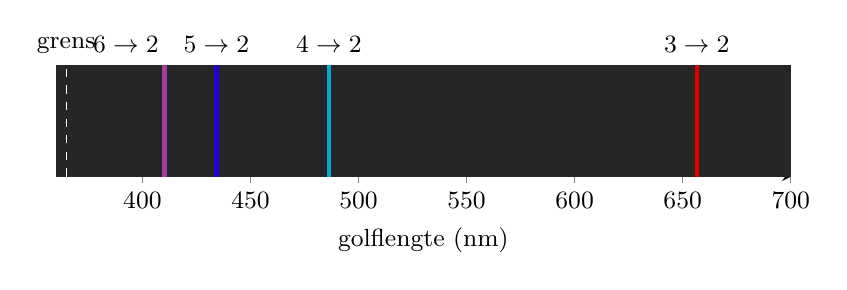
\begin{tikzpicture}
\begin{axis}[
  width=0.9\linewidth, height=3.0cm,
  xmin=360, xmax=700, ymin=0, ymax=1,
  axis x line=bottom, axis y line=none,
  xlabel={golflengte (nm)}, xtick={400,450,500,550,600,650,700},
  tick label style={font=\small}, label style={font=\small},
  clip=false]
\fill[black!85] (axis cs:360,0) rectangle (axis cs:700,1);
% line positions: figdata/out/bachelor-1-hydrogen-levels-balmer.dat
\draw[line width=1.6pt, red!90!black] (axis cs:656.5,0) -- (axis cs:656.5,1);
\draw[line width=1.6pt, cyan!80!green] (axis cs:486.3,0) -- (axis cs:486.3,1);
\draw[line width=1.6pt, blue!70!violet] (axis cs:434.2,0) -- (axis cs:434.2,1);
\draw[line width=1.6pt, violet!75] (axis cs:410.3,0) -- (axis cs:410.3,1);
\draw[white, dashed] (axis cs:364.7,0) -- (axis cs:364.7,1);
\node[font=\small, anchor=south] at (axis cs:364.7,1.02) {grens};
\node[font=\small, anchor=south] at (axis cs:656.5,1.02) {$3\to2$};
\node[font=\small, anchor=south] at (axis cs:486.3,1.02) {$4\to2$};
\node[font=\small, anchor=south] at (axis cs:434.2,1.02) {$5\to2$};
\node[font=\small, anchor=south east] at (axis cs:412,1.02) {$6\to2$};
\end{axis}
\end{tikzpicture}


{\small De balmerlijnen, berekend met de formule van Rydberg
(golflengten in vacuüm), op de zichtbare band. Verdere lijnen dringen zich
samen naar de reeksgrens bij \qty{364.7}{nm}, in het ultraviolet.}
\end{omfigure}

\begin{history}[Het atoom van Bohr, 1913]
In 1913 stelde Niels Bohr, een 28-jarige Deense natuurkundige die in
Manchester werkte, voor dat het elektron van waterstof alleen langs
bepaalde banen om de kern kon draaien, en dat er licht werd uitgezonden
wanneer het van de ene baan naar een lagere sprong. Zijn model gaf de
balmerlijnen exact, en ook de waarde van de rydbergconstante uit $h$,
$e$ en de massa van het elektron. De banen overleefden de
kwantummechanica van 1925--1926 niet, de gekwantiseerde niveaus wel. Bohr
kreeg in 1922 de Nobelprijs voor Natuurkunde.
\end{history}

\begin{omfigure}
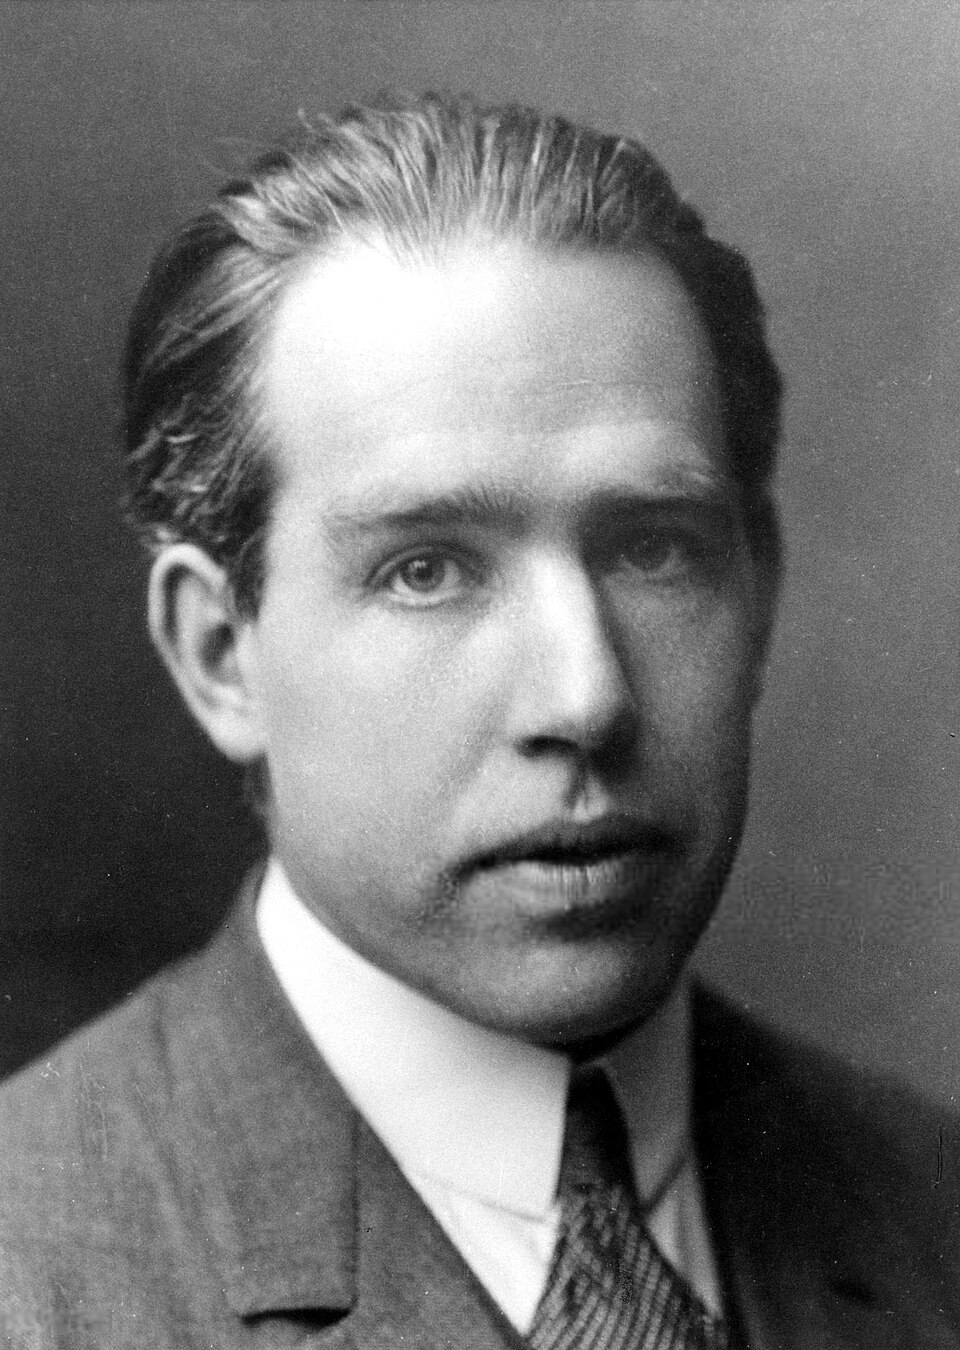
\includegraphics[width=0.26\linewidth]{images/book2/bohr.jpg}

{\small Niels Bohr (1885--1962), omstreeks 1922.}
\end{omfigure}

\section{Vier kwantumgetallen}

In een atoom met veel elektronen worden de energieën niet meer door één
enkele formule gegeven, maar elk elektron wordt nog steeds beschreven door
een klein stel gehele getallen, zijn kwantumgetallen.

\begin{definition}[Kwantumgetallen]\label{def:b1:quantum-numbers:quantum-number}
De toestand van een elektron in een atoom wordt aangeduid met vier
getallen:
\begin{itemize}
  \item het \emph{hoofdkwantumgetal}\index{hoofdkwantumgetal}
        $n = 1, 2, 3, \dots$, dat vooral de energie en de grootte bepaalt;
  \item het \emph{nevenkwantumgetal}\index{nevenkwantumgetal}
        (of azimutaal kwantumgetal) $l = 0, 1, \dots, n-1$, dat de vorm
        bepaalt; $l = 0, 1, 2, 3$ worden geschreven als s, p, d, f;
  \item het \emph{magnetisch kwantumgetal}\index{magnetisch kwantumgetal}
        $m_l = -l, -l+1, \dots, l$, dat de oriëntatie bepaalt ($2l + 1$
        waarden);
  \item het \emph{spinkwantumgetal}\index{spinkwantumgetal}
        $m_s = +\tfrac12$ of $-\tfrac12$, een intrinsieke eigenschap van
        het elektron, getekend als een pijl omhoog of omlaag.
\end{itemize}
\end{definition}

\begin{definition}[Atoomorbitaal, schil, subschil]\label{def:b1:quantum-numbers:orbital}
Een \emph{atoomorbitaal}\index{atoomorbitaal} is de
één-elektrontoestand die wordt aangeduid met de drie getallen
$(n, l, m_l)$; hij wordt getekend als één hokje, \omorbs{}. De orbitalen
met dezelfde $n$ vormen een
\emph{elektronenschil}\index{elektronenschil}; die met dezelfde $n$ en
$l$ vormen een \emph{subschil}\index{subschil}, benoemd met $n$ en de
letter van $l$: 2p is de subschil $n = 2$, $l = 1$, die uit drie
orbitalen bestaat ($m_l = -1, 0, 1$).
\end{definition}

\begin{remark}[Vormen]\label{rem:b1:quantum-numbers:shapes}
Een s-orbitaal is bolvormig; een p-orbitaal heeft twee lobben langs een
as, en de drie 2p-orbitalen wijzen langs $x$, $y$ en $z$. De wiskundige
beschrijving van die vormen --- golffuncties, hun radiale en hoekdelen,
hun knopen --- hoort bij het deel van jaar 2. In dit boek is een orbitaal
een hokje dat ten hoogste twee elektronen bevat.
\end{remark}

\begin{proposition}[Capaciteit van een subschil en van een schil]\label{prop:b1:quantum-numbers:capacity}
Een \omterm{def:b1:quantum-numbers:orbital}{subschil} met \omterm{def:b1:quantum-numbers:quantum-number}{nevenkwantumgetal} $l$ bevat $2l + 1$ orbitalen en kan
$2(2l + 1)$ elektronen bevatten: 2 in s, 6 in p, 10 in d, 14 in f. De
schil $n$ bevat $n^2$ orbitalen en kan $2n^2$ elektronen bevatten.
\end{proposition}

\begin{proof}
Bij een gegeven $l$ neemt $m_l$ de $2l + 1$ waarden van $-l$ tot $l$
aan, en elke orbitaal bevat twee elektronen met tegengestelde spin
(\cref{prop:b1:quantum-numbers:pauli} hieronder). Bij een gegeven $n$
loopt $l$ van $0$ tot $n - 1$, zodat het aantal orbitalen gelijk is aan
\[
  \sum_{l=0}^{n-1} (2l+1) = 2\,\frac{(n-1)n}{2} + n = n^2 ,
\]
en het aantal elektronen $2n^2$: 2, 8, 18, 32 voor $n = 1$ tot 4.
\end{proof}

\begin{example}[De derde schil]\label{ex:b1:quantum-numbers:third}
Voor $n = 3$: $l = 0$ (3s, één orbitaal), $l = 1$ (3p, drie orbitalen),
$l = 2$ (3d, vijf orbitalen, $m_l = -2, \dots, 2$): negen orbitalen en
ten hoogste 18 elektronen. Een elektron in 3d heeft bijvoorbeeld de
kwantumgetallen $(3, 2, -1, +\tfrac12)$.
\end{example}

\section{Configuraties opbouwen}

\begin{definition}[Elektronenconfiguratie]\label{def:b1:quantum-numbers:configuration}
De \emph{elektronenconfiguratie}\index{elektronenconfiguratie} van een
atoom of ion is de lijst van zijn bezette \omterm{def:b1:quantum-numbers:orbital}{subschillen}, met het aantal
elektronen in elk ervan als exponent geschreven: $1\text{s}^2 2\text{s}^2
2\text{p}^4$ voor zuurstof. De elektronen met de hoogste $n$, samen met
die van een onvolledig gevulde d- of \omterm{def:b1:quantum-numbers:orbital}{f-subschil}, zijn de
\emph{valentie-elektronen}\index{valentie-elektronen}; de andere zijn de
\emph{rompelektronen}\index{rompelektronen}. Een configuratie wordt
afgekort door de configuratie van het voorafgaande edelgas tussen
vierkante haken te schrijven: zuurstof is $[\ce{He}]\,2\text{s}^2 2\text{p}^4$.
\end{definition}

Drie regels geven de configuratie in de \omterm{def:b1:quantum-numbers:energy-level}{grondtoestand}.

\begin{proposition}[Uitsluitingsprincipe van Pauli]\label{prop:b1:quantum-numbers:pauli}
Twee elektronen van hetzelfde atoom hebben nooit dezelfde vier
kwantumgetallen. Eén orbitaal bevat dus ten hoogste twee elektronen, en
die hebben dan tegengestelde spin: \omorbs{ud}.
\end{proposition}
\admitted

\begin{proposition}[Regel van Klechkowski]\label{prop:b1:quantum-numbers:klechkowski}
In de \omterm{def:b1:quantum-numbers:energy-level}{grondtoestand} van een neutraal atoom worden de \omterm{def:b1:quantum-numbers:orbital}{subschillen} gevuld
in volgorde van toenemende $n + l$, en bij gelijke $n + l$ in volgorde van
toenemende $n$:
\[
  1\text{s},\ 2\text{s},\ 2\text{p},\ 3\text{s},\ 3\text{p},\ 4\text{s},\
  3\text{d},\ 4\text{p},\ 5\text{s},\ 4\text{d},\ 5\text{p},\ 6\text{s},\
  4\text{f},\ 5\text{d},\ 6\text{p},\ 7\text{s},\ 5\text{f},\ 6\text{d},\
  7\text{p}.
\]
\end{proposition}
\admitted

\begin{remark}[Een empirische regel]\label{rem:b1:quantum-numbers:klech-empirical}
De regel van Klechkowski (ook regel van Madelung genoemd) is een
samenvatting van waargenomen configuraties, geen wet: hij beschrijft de
volgorde waarin de \omterm{def:b1:quantum-numbers:orbital}{subschillen} zich vullen naarmate de kernlading
toeneemt. In een atoom met veel elektronen stoten de elektronen elkaar
af, zodat de energie van een \omterm{def:b1:quantum-numbers:orbital}{subschil} zowel van $l$ als van $n$ afhangt:
een 4s-elektron, dat een deel van zijn tijd dicht bij de kern doorbrengt,
komt in kalium en calcium onder 3d te liggen.
\end{remark}

\begin{omfigure}
\begin{tikzpicture}[font=\small, x=1.25cm, y=0.72cm]
  \foreach \n in {1,...,7} {
    \foreach \l/\s in {0/s,1/p,2/d,3/f} {
      \pgfmathtruncatemacro\ok{(\l<\n) && (\n+\l<=8)}
      \ifnum\ok=1
        \node[draw=black!50, rounded corners=2pt, minimum width=0.85cm,
          minimum height=0.5cm, fill=white] (s\n\l) at (\l,-\n) {\n\s};
      \fi
    }
  }
  \begin{scope}[on background layer]
  \foreach \la/\na/\lb/\nb in {0/1/0/1, 0/2/0/2, 1/2/0/3, 1/3/0/4, 2/3/0/5,
      2/4/0/6, 3/4/0/7, 3/5/1/7} {
    \draw[-{Stealth}, omDef, thick, opacity=0.8]
      ($(\la,-\na)+(0.5,0.42)$) -- ($(\lb,-\nb)+(-0.5,-0.42)$);
  }
  \end{scope}
  \node[anchor=west, align=left, font=\small] at (4.0,-2.5) {volg elke pijl,\\dan de volgende\\rechts ervan};
\end{tikzpicture}

{\small Het schema van Klechkowski. De \omterm{def:b1:quantum-numbers:orbital}{subschillen} met dezelfde $n + l$
liggen op één diagonaal; wie de diagonalen in volgorde doorloopt, krijgt
de opvulvolgorde 1s, 2s, 2p, 3s, 3p, 4s, 3d, 4p, 5s, \dots}
\end{omfigure}

\begin{proposition}[Regel van Hund]\label{prop:b1:quantum-numbers:hund}
Wanneer de elektronen van een \omterm{def:b1:quantum-numbers:orbital}{subschil} over meerdere orbitalen met
dezelfde energie verdeeld kunnen worden, heeft de \omterm{def:b1:quantum-numbers:energy-level}{grondtoestand} het
grootste aantal \emph{parallelle} spins: de elektronen bezetten
afzonderlijke orbitalen, met spin omhoog, voordat een orbitaal dubbel
bezet wordt.
\end{proposition}
\admitted

\begin{definition}[Ongepaard elektron]\label{def:b1:quantum-numbers:unpaired}
Een \emph{ongepaard elektron}\index{ongepaard elektron} is een elektron
dat alleen in zijn orbitaal zit. Een deeltje met ongepaarde elektronen
wordt door een magneet aangetrokken (het is paramagnetisch, een
eigenschap die in de natuurkunde bestudeerd wordt).
\end{definition}

\begin{method}[Een configuratie in de grondtoestand schrijven]\label{met:b1:quantum-numbers:configuration}
Zo schrijf je de configuratie van een atoom met atoomnummer $Z$:
\begin{enumerate}
  \item verdeel $Z$ elektronen over de \omterm{def:b1:quantum-numbers:orbital}{subschillen} in de volgorde van
        Klechkowski, en vul elke \omterm{def:b1:quantum-numbers:orbital}{subschil} (2, 6, 10, 14) vóór de
        volgende;
  \item schrijf het resultaat in volgorde van toenemende $n$ (3d bij
        $n = 3$ gegroepeerd), en kort af met de romp van het
        voorafgaande edelgas;
  \item teken voor de laatste, onvolledig gevulde \omterm{def:b1:quantum-numbers:orbital}{subschil} de hokjes en
        pas de regel van Hund toe om de \omterm{def:b1:quantum-numbers:unpaired}{ongepaarde elektronen} te tellen.
\end{enumerate}
\end{method}

\begin{example}[Koolstof, stikstof, zuurstof, ijzer]\label{ex:b1:quantum-numbers:examples}
De methode geeft voor vier atomen:
\begin{center}
\begin{tabular}{lllc}
\hline
atoom & configuratie & laatste \omterm{def:b1:quantum-numbers:orbital}{subschil} & ongepaard \\
\hline
\ce{C} ($Z = 6$) & $[\ce{He}]\,2\text{s}^2 2\text{p}^2$ & 2p: \omorbs{u,u,} & 2 \\
\ce{N} ($Z = 7$) & $[\ce{He}]\,2\text{s}^2 2\text{p}^3$ & 2p: \omorbs{u,u,u} & 3 \\
\ce{O} ($Z = 8$) & $[\ce{He}]\,2\text{s}^2 2\text{p}^4$ & 2p: \omorbs{ud,u,u} & 2 \\
\ce{Fe} ($Z = 26$) & $[\ce{Ar}]\,3\text{d}^6 4\text{s}^2$ & 3d: \omorbs{ud,u,u,u,u} & 4 \\
\hline
\end{tabular}
\end{center}
Voor ijzer vult de volgorde van Klechkowski 4s ($Z = 19, 20$) vóór 3d
($Z = 21$ tot 30); de configuratie wordt met 3d eerst geschreven.
% ledger: gs:Fe
\end{example}

\begin{omfigure}
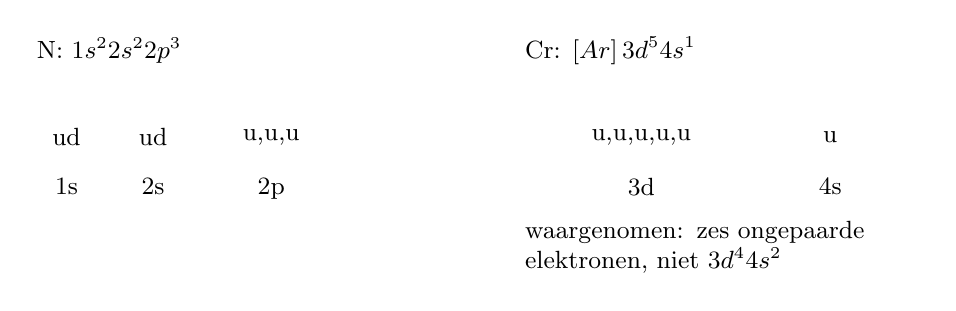
\begin{tikzpicture}[font=\small]
  \begin{scope}
    \node[anchor=west] at (0,2.4) {\ce{N}: $1\text{s}^2 2\text{s}^2 2\text{p}^3$};
    \node at (0.5,1.3) {\omorbs{ud}}; \node[below] at (0.5,0.9) {1s};
    \node at (1.6,1.3) {\omorbs{ud}}; \node[below] at (1.6,0.9) {2s};
    \node at (3.1,1.3) {\omorbs{u,u,u}}; \node[below] at (3.1,0.9) {2p};
  \end{scope}
  \begin{scope}[xshift=6.2cm]
    \node[anchor=west] at (0,2.4) {\ce{Cr}: $[\ce{Ar}]\,3\text{d}^5 4\text{s}^1$};
    \node at (1.6,1.3) {\omorbs{u,u,u,u,u}}; \node[below] at (1.6,0.9) {3d};
    \node at (4.0,1.3) {\omorbs{u}}; \node[below] at (4.0,0.9) {4s};
    \node[anchor=west, text width=5.0cm] at (0,-0.1) {waargenomen: zes ongepaarde elektronen, niet $3\text{d}^4 4\text{s}^2$};
\end{scope}
\end{tikzpicture}

{\small Kwantumhokjes. Elk hokje is één orbitaal; een pijl is één
elektron met zijn spin. Stikstof volgt de regel van Hund; chroom is een
van de uitzonderingen van \cref{prop:b1:quantum-numbers:exceptions}.}
\end{omfigure}

\section{Ionen, uitzonderingen en de vorm van het systeem}

\begin{proposition}[Configuraties van ionen]\label{prop:b1:quantum-numbers:ions}
Een eenatomig anion heeft de configuratie van het atoom, met de extra
elektronen op de volgende plaatsen van de volgorde van Klechkowski; een
kation van een hoofdgroepelement verliest de elektronen met de hoogste
$n$. Een kation van een overgangsmetaal verliest zijn $n$s-elektronen
\emph{vóór} zijn $(n-1)$d-elektronen: \ce{Fe^{2+}} is $[\ce{Ar}]\,3\text{d}^6$
en \ce{Fe^{3+}} is $[\ce{Ar}]\,3\text{d}^5$, niet $[\ce{Ar}]\,3\text{d}^4
4\text{s}^2$.
% ledger: gs:Fe2+, gs:Fe3+
\end{proposition}
\admitted


\begin{remark}[Opvulvolgorde is geen verwijderingsvolgorde]\label{rem:b1:quantum-numbers:order}
4s wordt in kalium en calcium vóór 3d gevuld, en toch wordt het in de
ionen van de overgangsmetalen het eerst geleegd. Dat is geen
tegenspraak: de volgorde van de energieën van de \omterm{def:b1:quantum-numbers:orbital}{subschillen} verandert
met de kernlading en het aantal elektronen, en in een atoom of ion van
een overgangsmetaal ligt de 3d-subschil onder 4s. De regel van
Klechkowski beschrijft alleen neutrale atomen.
\end{remark}

\begin{proposition}[Twee uitzonderingen in de eerste overgangsreeks]\label{prop:b1:quantum-numbers:exceptions}
De waargenomen configuraties in de \omterm{def:b1:quantum-numbers:energy-level}{grondtoestand} van chroom en koper zijn
\[
  \ce{Cr}: [\ce{Ar}]\,3\text{d}^5 4\text{s}^1, \qquad
  \ce{Cu}: [\ce{Ar}]\,3\text{d}^{10} 4\text{s}^1 ,
\]
in plaats van de $3\text{d}^4 4\text{s}^2$ en $3\text{d}^9 4\text{s}^2$
die de regel van Klechkowski voorspelt: een half gevulde of volle
\omterm{def:b1:quantum-numbers:orbital}{d-subschil} is bijzonder stabiel, en de niveaus 4s en 3d liggen dicht bij
elkaar.
% ledger: gs:Cr, gs:Cu
\end{proposition}


\begin{example}[Koper en zijn ionen]\label{ex:b1:quantum-numbers:copper}
\ce{Cu} is $[\ce{Ar}]\,3\text{d}^{10} 4\text{s}^1$; \ce{Cu+} is
$[\ce{Ar}]\,3\text{d}^{10}$, zonder \omterm{def:b1:quantum-numbers:unpaired}{ongepaard elektron}; \ce{Cu^{2+}} is
$[\ce{Ar}]\,3\text{d}^9$, met één. \ce{Zn^{2+}}, $[\ce{Ar}]\,3\text{d}^{10}$,
heeft er geen.
% ledger: gs:Cu+, gs:Cu2+, gs:Zn2+
\end{example}


\begin{proposition}[Configuraties en het periodiek systeem]\label{prop:b1:quantum-numbers:table}
Periode $n$ van het periodiek systeem begint met het vullen van $n$s en
eindigt met het vullen van $n$p. De \omterm{def:b1:quantum-numbers:orbital}{subschillen} die daartussen gevuld
worden, zijn volgens de regel van Klechkowski $(n-2)$f en $(n-1)$d. De
perioden bevatten dus $2, 8, 8, 18, 18, 32, 32$ elementen, en de
edelgassen hebben $Z = 2, 10,
18, 36, 54, 86, 118$.
\end{proposition}

\begin{proof}
De perioden 1 tot 3 bevatten alleen $n$s (en $n$p voor $n \ge 2$): $2$,
daarna tweemaal $2 + 6 = 8$. In de perioden 4 en 5 komt $(n-1)$d erbij:
$2 + 10 + 6 =
18$. In de perioden 6 en 7 ook $(n-2)$f:
$2 + 14 + 10 + 6 = 32$. De edelgassen sluiten elke periode af: $2$,
$2 + 8 = 10$, $18$, $18 + 18 = 36$, $54$, $54 + 32 = 86$, $118$.
\end{proof}

\begin{omfigure}
\omperiodictable[colour=blocks, legend]

{\small Het periodiek systeem, gekleurd naar de laatste \omterm{def:b1:quantum-numbers:orbital}{subschil} die
gevuld wordt: het s-, p-, d- en f-blok. De breedte van elk blok is de
capaciteit van zijn \omterm{def:b1:quantum-numbers:orbital}{subschil}, 2, 6, 10 en 14.}
\end{omfigure}

\section{Oefeningen}

\begin{exercise}[$\star$]\label{exo:b1:quantum-numbers:1}
Welke van deze viertallen $(n, l, m_l, m_s)$ kunnen een elektron in een
atoom beschrijven? Leg elke afwijzing uit.
(a) $(2, 2, 0, +\tfrac12)$; (b) $(3, 1, -1, -\tfrac12)$;
(c) $(1, 0, 0, 0)$; (d) $(4, 3, -3, +\tfrac12)$; (e) $(3, 0, 1, -\tfrac12)$.
\end{exercise}

\begin{exercise}[$\star$]\label{exo:b1:quantum-numbers:2}
Hoeveel orbitalen, en ten hoogste hoeveel elektronen, bevatten de
\omterm{def:b1:quantum-numbers:orbital}{subschillen} 3d, 4f en 5p, en de schil $n = 2$?
\end{exercise}

\begin{exercise}[$\star$]\label{exo:b1:quantum-numbers:3}
Schrijf de configuraties in de \omterm{def:b1:quantum-numbers:energy-level}{grondtoestand} van \ce{O}, \ce{P}, \ce{K},
\ce{Ca} en \ce{Br} ($Z = 8, 15, 19, 20, 35$) voluit en afgekort, en geef
van elk het aantal \omterm{def:b1:quantum-numbers:configuration}{valentie-elektronen}.
\end{exercise}

\begin{exercise}[$\star$]\label{exo:b1:quantum-numbers:4}
Teken de kwantumhokjes van de valentiesubschillen van stikstof, zwavel
en chloor, en tel hun \omterm{def:b1:quantum-numbers:unpaired}{ongepaarde elektronen}.
\end{exercise}

\begin{exercise}[$\star\star$]\label{exo:b1:quantum-numbers:5}
Geef de configuraties van \ce{Na+}, \ce{Mg^{2+}}, \ce{Al^{3+}}, \ce{F-},
\ce{O^{2-}}, \ce{Cl-}, \ce{S^{2-}} en \ce{Ca^{2+}}. Met welk edelgas is
elk ervan iso-elektronisch?
\end{exercise}

\begin{exercise}[$\star\star$]\label{exo:b1:quantum-numbers:6}
Schrijf de configuraties van \ce{Ti^{2+}}, \ce{Mn^{2+}}, \ce{Co^{2+}},
\ce{Ni^{2+}} en \ce{Zn^{2+}} ($Z = 22, 25, 27, 28, 30$) en geef van elk
het aantal \omterm{def:b1:quantum-numbers:unpaired}{ongepaarde elektronen}.
\end{exercise}

\begin{exercise}[$\star\star$]\label{exo:b1:quantum-numbers:7}
Bereken de energie en de golflengte van het foton dat bij de overgang
$4 \to 3$ van waterstof wordt uitgezonden. In welk deel van het spectrum
ligt het? Neem $E_R = \qty{13.6}{eV}$ en $hc = \qty{1240}{eV.nm}$.
\end{exercise}

\begin{exercise}[$\star\star$]\label{exo:b1:quantum-numbers:8}
Identificeer de elementen waarvan de configuratie in de \omterm{def:b1:quantum-numbers:energy-level}{grondtoestand}
eindigt op (a) $3\text{s}^2 3\text{p}^4$; (b) $4\text{s}^2 3\text{d}^{10} 4\text{p}^5$;
(c) $5\text{s}^1$; (d) $4\text{s}^2 3\text{d}^3$. Geef de vier
kwantumgetallen van één elektron van de laatste \omterm{def:b1:quantum-numbers:orbital}{subschil} van (a).
\end{exercise}

\begin{exercise}[$\star\star$]\label{exo:b1:quantum-numbers:9}
Leg met de regel van Klechkowski uit waarom het negentiende elektron van
kalium in 4s terechtkomt en niet in 3d, en waarom periode 3 acht
elementen bevat en geen achttien.
\end{exercise}

\begin{exercise}[$\star\star\star$]\label{exo:b1:quantum-numbers:10}
Een ion met één enkel elektron en een kern met lading $Ze$ heeft de
niveaus $E_n = -Z^2 E_R/n^2$ (aangenomen). Bereken voor \ce{He+}
($Z = 2$) de ionisatie-energie en de golflengte van de overgang $2 \to 1$.
Vergelijk met waterstof.
\end{exercise}

\begin{exercise}[$\star\star\star$]\label{exo:b1:quantum-numbers:11}
Zeg van elke configuratie of het een \omterm{def:b1:quantum-numbers:energy-level}{grondtoestand}, een \omterm{def:b1:quantum-numbers:energy-level}{aangeslagen
toestand} of onmogelijk is, en waarom: (a) $1\text{s}^2 2\text{s}^1 2\text{p}^1$;
(b) $1\text{s}^2 2\text{s}^2 2\text{p}^7$; (c) $1\text{s}^2 2\text{p}^2$;
(d) $[\ce{Ne}]\,3\text{s}^2 3\text{p}^3$; (e) $1\text{s}^3$.
\end{exercise}

\begin{exercise}[$\star\star\star$]\label{exo:b1:quantum-numbers:12}
IJzer(III)zouten worden sterker door een magneet aangetrokken dan
ijzer(II)zouten, en zinkzouten helemaal niet. Rangschik \ce{Fe^{2+}},
\ce{Fe^{3+}}, \ce{Mn^{2+}}, \ce{Cu^{2+}} en \ce{Zn^{2+}} naar het aantal
\omterm{def:b1:quantum-numbers:unpaired}{ongepaarde elektronen}, en verklaar de waarneming, in de veronderstelling
dat de aantrekking met dat aantal toeneemt.
\end{exercise}

\section{Probleem: lijnen van een lamp, en een wereld met drie spins}

\begin{problem}[{Weekendprobleem --- van de vier lijnen van een
waterstoflamp naar de lengte van de perioden, en hoe het periodiek systeem
eruit zou zien als een elektron drie spintoestanden had}]
\label{pb:b1:quantum-numbers:1}
Neem overal $E_R = \qty{13.6}{eV}$ en $hc = \qty{1240}{eV.nm}$. De
zichtbare band loopt van ongeveer 400 tot \qty{700}{nm}.

\medskip
\noindent\textbf{Deel I --- De waterstoflamp.}
\begin{enumerate}
  \item Bereken de energieën $E_1$ tot $E_4$ van het waterstofatoom.
  \item Bereken de energie en de golflengte van het foton dat bij de
        overgang $3 \to 2$ wordt uitgezonden. Welke kleur heeft het?
  \item Bereken de golflengten van de overgangen $4 \to 2$, $5 \to 2$
        en $6 \to 2$.
  \item Waarom toont een waterstoflamp precies vier zichtbare lijnen?
        Bereken de golflengte van $7 \to 2$ om het antwoord te staven.
  \item Bereken de reeksgrens van de balmerreeks.
  \item Bereken de golflengte van de eerste lymanlijn, $2 \to 1$. Waarom
        is die niet te zien?
  \item Wat is de grootste golflengte van een foton dat een waterstofatoom
        in de \omterm{def:b1:quantum-numbers:energy-level}{grondtoestand} kan ioniseren?
\end{enumerate}

\medskip
\noindent\textbf{Deel II --- Toestanden tellen.}
\begin{enumerate}[resume]
  \item Som de waarden van $l$ en $m_l$ op voor $n = 3$; hoeveel orbitalen
        bevat de schil?
  \item Toon aan dat de schil $n$ $2n^2$ elektronen bevat; pas toe op
        $n = 4$.
  \item Schrijf de volgorde van Klechkowski op tot 7p.
  \item Leid de lengten van de zeven perioden af.
  \item Leg uit waarom de 3d-subschil niet in periode 3 voorkomt.
  \item Leid de atoomnummers van de edelgassen af.
\end{enumerate}

\medskip
\noindent\textbf{Deel III --- De overgangsmetalen.}
\begin{enumerate}[resume]
  \item Schrijf de configuratie van ijzer ($Z = 26$) en teken zijn
        3d-hokjes. Hoeveel \omterm{def:b1:quantum-numbers:unpaired}{ongepaarde elektronen} zijn er?
  \item Dezelfde vragen voor \ce{Fe^{2+}} en \ce{Fe^{3+}}. Welk van de twee
        heeft een half gevulde \omterm{def:b1:quantum-numbers:orbital}{subschil}?
  \item De waargenomen configuratie van chroom is $[\ce{Ar}]\,3\text{d}^5
        4\text{s}^1$. Vergelijk met de voorspelling, en tel in beide
        gevallen de \omterm{def:b1:quantum-numbers:unpaired}{ongepaarde elektronen}.
  \item Geef de configuraties van \ce{Cu}, \ce{Cu+} en \ce{Cu^{2+}}.
  \item Welk van \ce{Cu+} en \ce{Cu^{2+}} heeft \omterm{def:b1:quantum-numbers:unpaired}{ongepaarde elektronen}?
  \item Welk van \ce{Sc^{3+}}, \ce{Ti^{3+}}, \ce{Mn^{2+}} ($Z = 21, 22, 25$)
        heeft de meeste \omterm{def:b1:quantum-numbers:unpaired}{ongepaarde elektronen}?
\end{enumerate}

\medskip
\noindent\textbf{Deel IV --- Een wereld met drie spins.}
Stel je een heelal voor waarin $n$, $l$ en $m_l$ dezelfde regels volgen
als in het onze, de volgorde van Klechkowski ongewijzigd is en het
uitsluitingsprincipe geldt, maar het spingetal $m_s$ drie waarden kan
aannemen.
\begin{enumerate}[resume]
  \item Hoeveel elektronen kan één orbitaal bevatten? Een \omterm{def:b1:quantum-numbers:orbital}{subschil} met
        getal $l$? Een schil $n$?
  \item Geef de capaciteiten van 1s, 2s, 2p, 3s en 3p.
  \item Een edelgas sluit een periode af met een volle \omterm{def:b1:quantum-numbers:orbital}{p-subschil} (of 1s
        voor het eerste). Wat is het atoomnummer van het eerste edelgas?
  \item Welk atoomnummer zou zich gedragen als een alkalimetaal, met één
        enkel elektron voorbij het eerste edelgas?
  \item Hoeveel elementen zou de tweede periode bevatten?
  \item Bereken het atoomnummer van het tweede edelgas van deze wereld.
\end{enumerate}
\end{problem}
